%==================================================================================================
%   LUKES THESIS TEMPLATE 1.2
%   -------------------------
%   This template is based upon the offcial IMM PhD Thesis template, it is enhanced with a number
%   of new features and a number of errors have fixed. This template is intended to be complied to
%   PDF using PDFLATEX and is tested using the MiKTeX 2.9 LaTeX distribution.
%   It is based on the official DTU-IMM Thesis template by Finn Kuno Christensen in 2009.
%   Small bugfixes by Kasper Laursen in 2012.
%   -------------------------
%   Last Updated: 2012-09-19
%   Contact: lthhe@imm.dtu.dk
%==================================================================================================
%
% 


%==================================================================================================
% DOCUMENT SETUP
%==================================================================================================



\documentclass[10pt,twoside]{book}                  %Official DTU-IMM Thesis document setup



%
%Set to 'print' for printed version, use 'net' for online version
\def\thesisversion{print}
%
%==================================================================================================
% PACKAGES
%==================================================================================================
\usepackage{Thesis}                             %Import Thesis base style
%input{PhDMacros}                                   %Thesis specific macros
%
%==================================================================================================
% THESIS PROPERTIES (Modifiy these fields with your details)
%==================================================================================================
\def\thesisauthor{Constantina Ioannou}                     %Author
\def\thesistitle{Mining a Developer's Workflow from IDE Usage}               %Title
\def\thesishandin{1 March}			                %Submission date (Day-Month}
\def\thesisdegree{MSc}                            %Degree ('B.Eng', 'B.Sc.', 'M.Sc.' or 'PhD')
\def\thesisyear{2018}                               %Submission year
\def\thesisnumber{73}                             %DTU-IMM Serial number (do not include year)
\def\thesisISSN{0000-0000}                          %ISSN number
\def\thesiskeywords{Keywords are, comma separated}  %PDF keywords
\derivethesisprops                                  %Derive dependent properties
%
%==================================================================================================
% SECTION NUMBERING SETUP
%==================================================================================================
\setcounter{tocdepth}{2}                            %2 adds sections up to subsections
\setcounter{secnumdepth}{3}                         %Subsubsections get a number when this is 3
%
%==================================================================================================
% THESIS STRUCTURE  (Modifiy to include more chapters etc)
%==================================================================================================
\begin{document}
%------------------------
%Pre-frontmatter material
%------------------------
\prefrontmatter
%--------------------
%Frontmatter material
%--------------------
\frontmatter
\pagenumbering{roman}                               %Set frontmatter numbering style
\chapter{Abstract}



Software developers interact with integrated development environments (IDEs) by issuing commands that execute various programming tools, from source code formatters to build tools. Several studies has shown that despite the usefulness of provided tools and capabilities to perform tasks such as: navigating among classes and methods, continuous compilation, code refactoring and integrated debugging, IDEs usually tend to overload developers resulting a chaotic state. In other words, commonly developers spend time shifting between several artifacts of the working environment in order to reach their goal, and this repeated process increases the complexity of identifying the relevant information to solve their assignment. 

For this reason, an assortment of usage metrics plugins to gather developers' activity have been developed in an attempt to understand a developers' workflow. Understanding the workflow, as well as the skillset and experience of a developer is the first step into improving their productivity and reducing the unneccessary complexity created within IDEs. 

In this work, we analyze and provide an overview of available existing plugins for recording a developer's interaction within an IDE and we further enhance a tool in order to capture, mine and analyze the process of software developement. We aim to contribute information for modelling an automatic activity detection tool capable of tracking the workflow of developers’ activity which potentially will be used as input in later studies for a reconfiguration program supporting the developer.

In more depth, this thesis will provide an overview of contextual factors and an analysis of how they can be achieved using already existing plugins that allow recording developers’ activity within Eclipse IDE. In addition, is expected to uncover and characterise developer’s workflow.
\todo{write}
%we also examine the link between programmer's interaction and some of the contextual factors of software development
%In this work, i'd like to propose a model to present the user interactions I gather from the IDE. in parallel with the process mining we gonna make

                                   %English summary of Thesis
\markboth{}{}                                       %Set headings (left)(right)
\chapter{Preface}
\vspace{-15mm}
This thesis was carried out at the department of DTU Compute, at the Technical University of Denmark, in fulfilment of the requirements for acquiring an M.Sc. in Computer Science and Engineering.\\
The goal of this project was to collect data on how developers interact with an IDE while developing software and to mine developers' workflows from IDE usage using process mining techniques. 

This report describes the project itself and discusses concepts involved. Further, analyses in detail the software which was selected for expantion and features that were developed during this project. Finally, presents the results of mining developers' interactions according to their IDE usage.
%==================================================================================================
% SIGNATURE AREA
%==================================================================================================
%\vspace{-5mm}
\todo{add signature}
% \begin{center}
%     \hspace{20mm} Lyngby, \thesishandin-\thesisyear
%     \newline
%   %Update signature image file in line below
%     \includegraphics[scale=0.1]{figures/Signature.pdf}
% \end{center}
% \begin{flushright}
%     \thesisauthor
% \end{flushright}
% % % EOF % % %
                                     %Preface
\markboth{}{}                                       %Set headings (left)(right)
\chapter{Acknowledgements}

My deepest thanks go to my advisor, Barbara Weber. Throughout these months, Barbara gave me the freedom for exploring an unkown field, challenged my findings, and offered advices whenever needed. Barbara taught me the importance of software methodologies and helped me to evolve my experience with agile environments: by narrowing down ideas and being selective over the most feasible ones. All these advices have been invaluable. 
I also thank my co-supervisor Andrea Burattin for his time and feedback. Andrea shared his knowledge regarding process mining and his questions and suggestions have enabled me to view this work from a wider perspective.
Furthermore I would like to express my gratitude to my family and friends who showed patience and were supportive during moments of frustrations.

A great thank you to everyone who believed in me! 

                            %Acknowledgements
\markboth{}{}                                       %Set headings (left)(right)

\newacronym{pde}{PDE}{Plug-in Developer Environment}
\newacronym{rsse}{RSSE}{Recommendation System in Software Engineers}

\newacronym{ide}{IDE}{Integrated Development Environment}


%------------------
% Table of contents
%------------------
\newpage\mbox{}\newpage
\chaptermark{Contents}
\pdfbookmark{\contentsname}{toc}
\renewcommand{\sectionmark}[1]{\markright{#1}}
\sectionmark{Contents}
\addtolength{\parskip}{-\baselineskip}
\tableofcontents
\addtolength{\parskip}{\baselineskip}
\renewcommand{\sectionmark}[1]{\markright{\thesection\ #1}}


%-------------
% Main content
%-------------
\mainmatter
\chapter{Introduction}

Programming is a really complex procedure and requires a great amount of human memory. Although modern program development environments have begun to recognize the complexity and the memory requirements of programmers, none of these tools are able to take into account the programmers' cognition. \addref{Chris Parnin and Spencer Rugaber. Programmer information needs after memory failure. In ICPC ’12: Proceedings of the 20 Interaction Conference on Program Comprehension, pages 123–132, 2012.
} Therefore the process of software development doesn't feel any better than it did a generation ago. Previous research focuses on understanding how developers operate to complete their jobs: how they keep their tasks structured, the strategies they apply, the tools they use


Several studies has shown that, despite the usefulness of provided tools and capabilities to perform tasks such as navigating among classes and methods, continuous compilation, code refactoring and integrated debugging, IDEs usually tend to overload de- velopers resulting a chaotic state. In other words, commonly developers spend time shifting between several artifacts of the working environment in order to reach their goal, and this repeated process increases the complexity of identifying the relevant information to solve their assignment. 

Yet researchers pointed out certain aspects of the problem still the workflow and the way a programmer might think at a particular moments is still a mystery.

in order to improve the environments available we have although to understand these aspects.

ides aim to help the user however often they create a general chaos with all the navigation the studies of .. and the Cognition studies and models strategies top down bottom up, 

previous research of understanding the workflow of a developer is done by ... 

previous research of attempting to extracct user activities from \gls{ide} ... 

Abstract—Developers use the Integrated Development Environ-
ment (IDE) to develop a system at hand, by reading, understand-
ing, and writing its source code. They do so by exploiting the tools

and facilities provided by the IDE. This also allows them to build
a mental model of the system to perform informed changes. It is
however not clear how and when developers use which facility
and tool, and to what extent the current services o↵ered by the
IDE appropriately support the navigation.
We present an approach to visualize the activities of developers
within the IDE, implemented in a tool: DFlow. DFlow records
all IDE interactions that occur during a development session and



By better understanding actual work practices, looking for patterns in them, and in performing empirical studies based on this knowledge, we can better address how to create the next generation of supporting tools for software developers.

Previous research of understanding how software developers do their jobs has focused mainly on studies of programmer cognition and work practices. Cognition studies try to ex- plore the cognitive models, strategies, and patterns used by developers performing program comprehension. Mostly based on laboratory experiments, these studies have shown that programmers apply multiple comprehension strategies, such as top-down [Bro77], bottom- up [Pen87] , and integrated [vMV95], and also that patterns in the code, such as beacons [Bro83, GC91], plays an important role in comprehension. These findings have guided the design of some research development tools (e.g., Shrimp [SBM01]) in supporting program comprehension. The study of developer work practices, on the other hand, focuses on a big picture of industrial developers working in the context of realistic development tasks. Sur- veys, diaries, interviews, and other methods have led to several surprising insights about work practice; for example, Singer et al. found that developers spend significant effort on
1
searching for code elsewhere in the system that relates in some way to the code they are working on [SLVN97]. Seaman found that the information sources that developers rely on most are source code, colleagues, and various development artifact repositories [Sea02]. These findings suggest that supporting improved information searching, interruption man- agement, and repository mining can be helpful to programmers.
%In this chapter we introduce some key aspects of Real-Time Systems (RTS), starting from the computational model. We then discuss \textit{timing analysis} and Worst-Case Execution Time (WCET) calculation. After that we introduce \textit{time-composability} and how important that property is. In Section the role of a Real-Time Operating System (RTOS) is described and some examples are presented. In the end the T-CREST project and platform are briefly described.


\section{The problem}

Although, the mentioned findings are a bit irrelevant because we are awesome

A fine-grained understanding of developers 
a fine-grained understanding of industrial programmers working in an industrial context remains limited. Cognitive studies often involve student programmers working on small problems. It is hard to generalize from such small-scale studies to industrial software development practice, where developers typically have a much larger code base and more complicated tasks to consider, and where they will be ultimately be held accountable for their decisions. Detecting high-level comprehension strategies has been the main focus of cognitive studies. But detailed work patterns — such as what artifacts are usually used for solving certain typical sub-tasks, and what relationships exist between those artifacts — remain mostly unexplored. Moreover, the relation between programmers’ work and contextual factors is poorly understood. As shown in Figure 1.1, driven by maintenance tasks, programmers interact with artifacts of a software system using tools in the work domain. 

Tasks may largely determine which parts of the software system are relevant, but other factors in software development, such as the expertise level of programmer, the design of the software system, the features of the tool, and interruptions during tasks, may all affect programmer’s detailed work pattern. To understand how industrial software developers perform their job — and how we can help them do better — we should not ignore these contextual factors.

\section{The approach}
\section{Integrated Development Environment}
	%\todo{list available and discuss}
	%\todo{paragraph why we choose eclipse}
	%\todo{programmer workflow within IDE}
\section{Structure of thesis}
                                  %Introduction
\chapter{\gls{ide}}\label{cha:IDEs}

%\section{Integrated Development Environment}
	%\todo{list available and discuss}
	%\todo{paragraph why we choose eclipse}
During programming tasks developers often interact with a variety of facilities and tools: browsers, \gls{ide}s, mail clients, virtual machines, etc. All these interactions are of high significance when it comes to understand the workflow of a developer. An \gls{ide} is very personal and therefore analysing developers' behavior is feasible. 

This chapter begins with an introduction to the history of \gls{ide}s to support their importance and a description of their future is given. Further, the main focus is the analysis and discussion of possible interaction with today's \gls{ide}s.

\section{Quick \gls{ide} History}

An \gls{ide} is a software application which aims to improve developers' productivity by facilitating application development. It consolidates the basic tools developers need to write and test software. Typically, an \gls{ide} consists of a source code editor, a compiler, a debugger and build automation tools. According to \addref{reference:} 
%https://www.veracode.com/security/integrated-development-environments} 
the idea behind \gls{ide} was realeased as Turbopascal which integrated an editor and a compile. However many believe Microsoft's Visual Basic (VB), launched in 1991 was the first real \gls{ide}, and by the time it was relatively easy to learn and use.

Over the years several \gls{ide}s have been implemented and released. \gls{ide}s offered remarkable advantages to developers mentioned in \addref{reference:}
% https://www.veracode.com/security/integrated-development-environments} 
and \addref{reference:} for example: %\addref{http://vantageonesoftware.com/advantages-disadvantages-integrated-development-environment/} for example: 
\begin{itemize}
\item Reducing the setup up time required to configure multiple development tools, 
\item Increasing development speed and efficiency by providing instant feedback for syntax errors or code insights,
\item Increasing program management by organising resources, providing a virtual representation of the project, and automatically adding appropriate imports. 
\item Increasing the quality of programs by offering the ability for debugging, testing and source control.
\end{itemize}


Overal these advantages of using an \gls{ide} have endorsed the productivity of a developer. Today, according to the Top IDE index \addref{reference:github}
%https://pypl.github.io/IDE.html}
, a ranking created by analysing how often \gls{ide}s are searched on Google, the 3 most used tools employed to develop source code are Eclipse, Visual Studio, Android Studio. Although \gls{ide}s are stricking through the top 3, it is noticable that a significant amount of developers prefer to use highly configurable text editors such as Vim and Sublime Text. The different types of code, specific languages, cloud based, mobile application, apple or microsoft development, led \gls{ide}s to expand in a variety of directions. Consequently not all \gls{ide}s offer the same capabilities and the same collection of tools. Therefore one must be selective when choosing an \gls{ide}, in accordance to its development task and requirements. 

Even though that \gls{ide}s are highly helpful to a developer, they lack effective support to browse between complex relationships between source code elements. This implies that developers spend 30\% their time navigating through a chaotic environment and therefore their productivity is being reduced as supported by \addref{Taming the IDE with Fine-grained Interaction Data}. \addref{Autumn leaves} and \addref{An explatory study}

%D. Roethlisberger, O. Nierstrasz, and S. Ducasse, Autumn leaves:
%Curing the window plague in IDEs, in Proceedings of WCRE (16th
%Working Conference on Reverse Engineering), 2009, pp. 237–246.} 

%{A. J. Ko, B. A. Myers, M. J. Coblenz, and H. H. Aung, An exploratory study of how developers seek, relate, and collect relevant information
%during software maintenance tasks, IEEE Transactions on Software Engineering, vol. 32, no. 12, pp. 971–987, 2006.}.


For this thesis, in an attempt to understand the developers' workflow the extraction of user interactions with an \gls{ide} is required. The decision to analyse and develop for Eclipse \gls{ide} was taken for a vast amount of reasons listed in \ref{cha:TheEclipseIDE}.



\section{Interactions within \gls{ide}}

\gls{ide}s are highly used by developers nowadays to develop and maintain a software. Developers use \gls{ide} to read, navigate, understand and write code. In more detail the developer interacts with \gls{ide} through low level events such as: mouse clicks and keyboard shortcuts but also high level events facilitated by the tools provided in the toolbar such as: refactoring, debugging, navigating, testing, inspecting as mentioned in \addref{An explatory study}
and \addref{How Much Integrated Development Environments Improve Productivity}. 
%{A. J. Ko, B. A. Myers, M. J. Coblenz, and H. H. Aung, An exploratory study of how developers seek, relate, and collect relevant informationduring software maintenance tasks, IEEE Transactions on Software Engineering, vol. 32, no. 12, pp. 971–987, 2006.} 
A high level event is a series of low level events. In other words the toolbar allows the developer to code, compile and execute source code without having to follow manually these steps.  An example is the process of renaming a class within a large project. \gls{ide} provides contextual menues enabling fast and efficient changes where otherwise a series of low level events: editing several classes, compiling and error seeking, executing and testing the correctness after the change should be done manually.

	\begin{figure}[!ht]
		\begin{center}
		 
        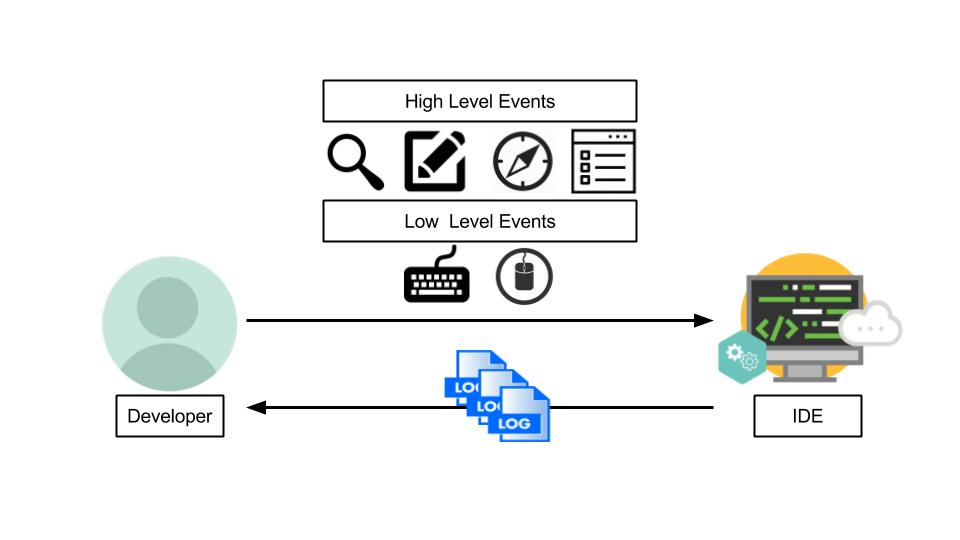
\includegraphics[width=\textwidth]{figures/ch1a_dev_ide.jpg}
		\end{center}
		\caption{Flow of usage data between developer and \gls{ide}.}
		\label{fig:ch1a_dev_ide}
	\end{figure}

According to \addref{Visualizing the Workflow of Developers} and \addref{Capturing and Exploiting IDE Interactions} by gathering all the IDE usage data provides an additional view of what the workflow of a developer is to solve a certain task.
A task (implementing a class, correcting an error) is consisting of a series of high and low level events  These interaction events are called usage data \addref{A Practical Guide to Analyzing IDE Usage Data} and they are an essential element for this thesis. All the usage data generated by the activity of a developer within an \gls{ide} are recorded. The developer initiates the different interactions and \gls{ide} responds back with logging particular events. The model in \ref{fig:ch1a_dev_ide} shows the exchange of usage data between developer and \gls{ide}.

\section{The usage data model for logs} 

\chapter{The Eclipse IDE}\label{cha:TheEclipseIDE}

In the following chapter a general overview of Eclipse framework and its most prominent components is provided. A description and analysis of available plug-ins from which essential information could be captured is presented. Last but not least a great amount of focus is given on a specific plug-in called Rabbit, which is used and enhanced throughout the thesis.  

%\todo{ide eclipse plug-ins, available what are useful, present all, write adv and dis. describe contextual factors that can be achieved, describe how programmers work within this ide. }
%\todo{focus on rabbit specia chapter explain why to choose that, positive negative, limitations. provide class diagram and explanation, name the issues}

\section{Eclipse}
\label{sec:TheEclipseIDE:eclipse}
Eclipse workbench is a powerful UI framework for \gls{ide}s fairly used by several developers: to primarily develop Java applications or even to develop in other programming languages, and to also develop documents and packages for other softwares. It provides several services for highly integrated and extensible user interfaces. Eclipse fulfills the requirement of an entire product developer team to use one platform where all their tools integrate and work together. This is one of the main reasons Eclipse is still the top \gls{ide} available \addref{top index ide}

The standard SDK Eclipse distribution contains a base workspace with certain functionalities, Java Developemnt tooling plug-ins and layout. Thereafter additional plug-ins can be included or created to allow the extension of the workspace. As a result Eclipse can become a multifunction framework to be used for: Embedded programming, C++ programming, javaBeans, Java application, websites, or even develop additional Eclipse plug-ins, etc. The plug-ins can be removed or replaced according to the needs and preferences of developers.

Even though Eclipse framework started as a replacement for Visual Age for Java from IBM \addref{ wikipedia}, it became an open platform for integrating tools, editors, views and plug-ins. Its source code is freely available and anyone can 
contribute by building their own new plug-ins or by engaging in discussions regarding integrated tools.

The most significant reasons of selecting the Eclipse \gls{ide} as a tool for gathering information for processing developers' workflow are: 
\begin{itemize}

\item It is the top ranked used \gls{ide} by developers \addref{ BOOK} and \addref{the top 10 index},
\item It is a home for tools, where you can build and intergrate your own \addref{ the book},
\item It is an open source framework, features and plug-ins are available online, the execution and source code files \addref{the book},
\item It is an open source Community \addref{eclipse.org}, collection of technical professionals with a common interest in using and contributing in the evolution of the platform.
\end{itemize}  

\section{Eclipse User Interface}
\label{sec:TheEclipseIDE:ui}
\subsection{Eclipse UI as Application Developer}
\addref{The eclipse foundation. eclipse documentation:release oxygen. online url// eclipse.org} 
Eclipse framework consists of workbench windows, which have integrated basic elements such as active perspectives, editors, views and menus.

When starting up Eclipse, if its a newly initiated greets the developer with a welcoming screen, otherwise the previously workspace is loaded. Figure \ref{fig:eclipse_worspace} displays a standard Eclipse setup for a Java \gls{ide}. 

A \textit{perspective} has its own a set of elements views and editors and menus along with a adaptable personalized layout for specific tasks such as debugging a program. 
%\label{sec:TheEclipseIDE:menusviewsandeditors}
	\begin{figure}[!ht]
		\begin{center}
		 
        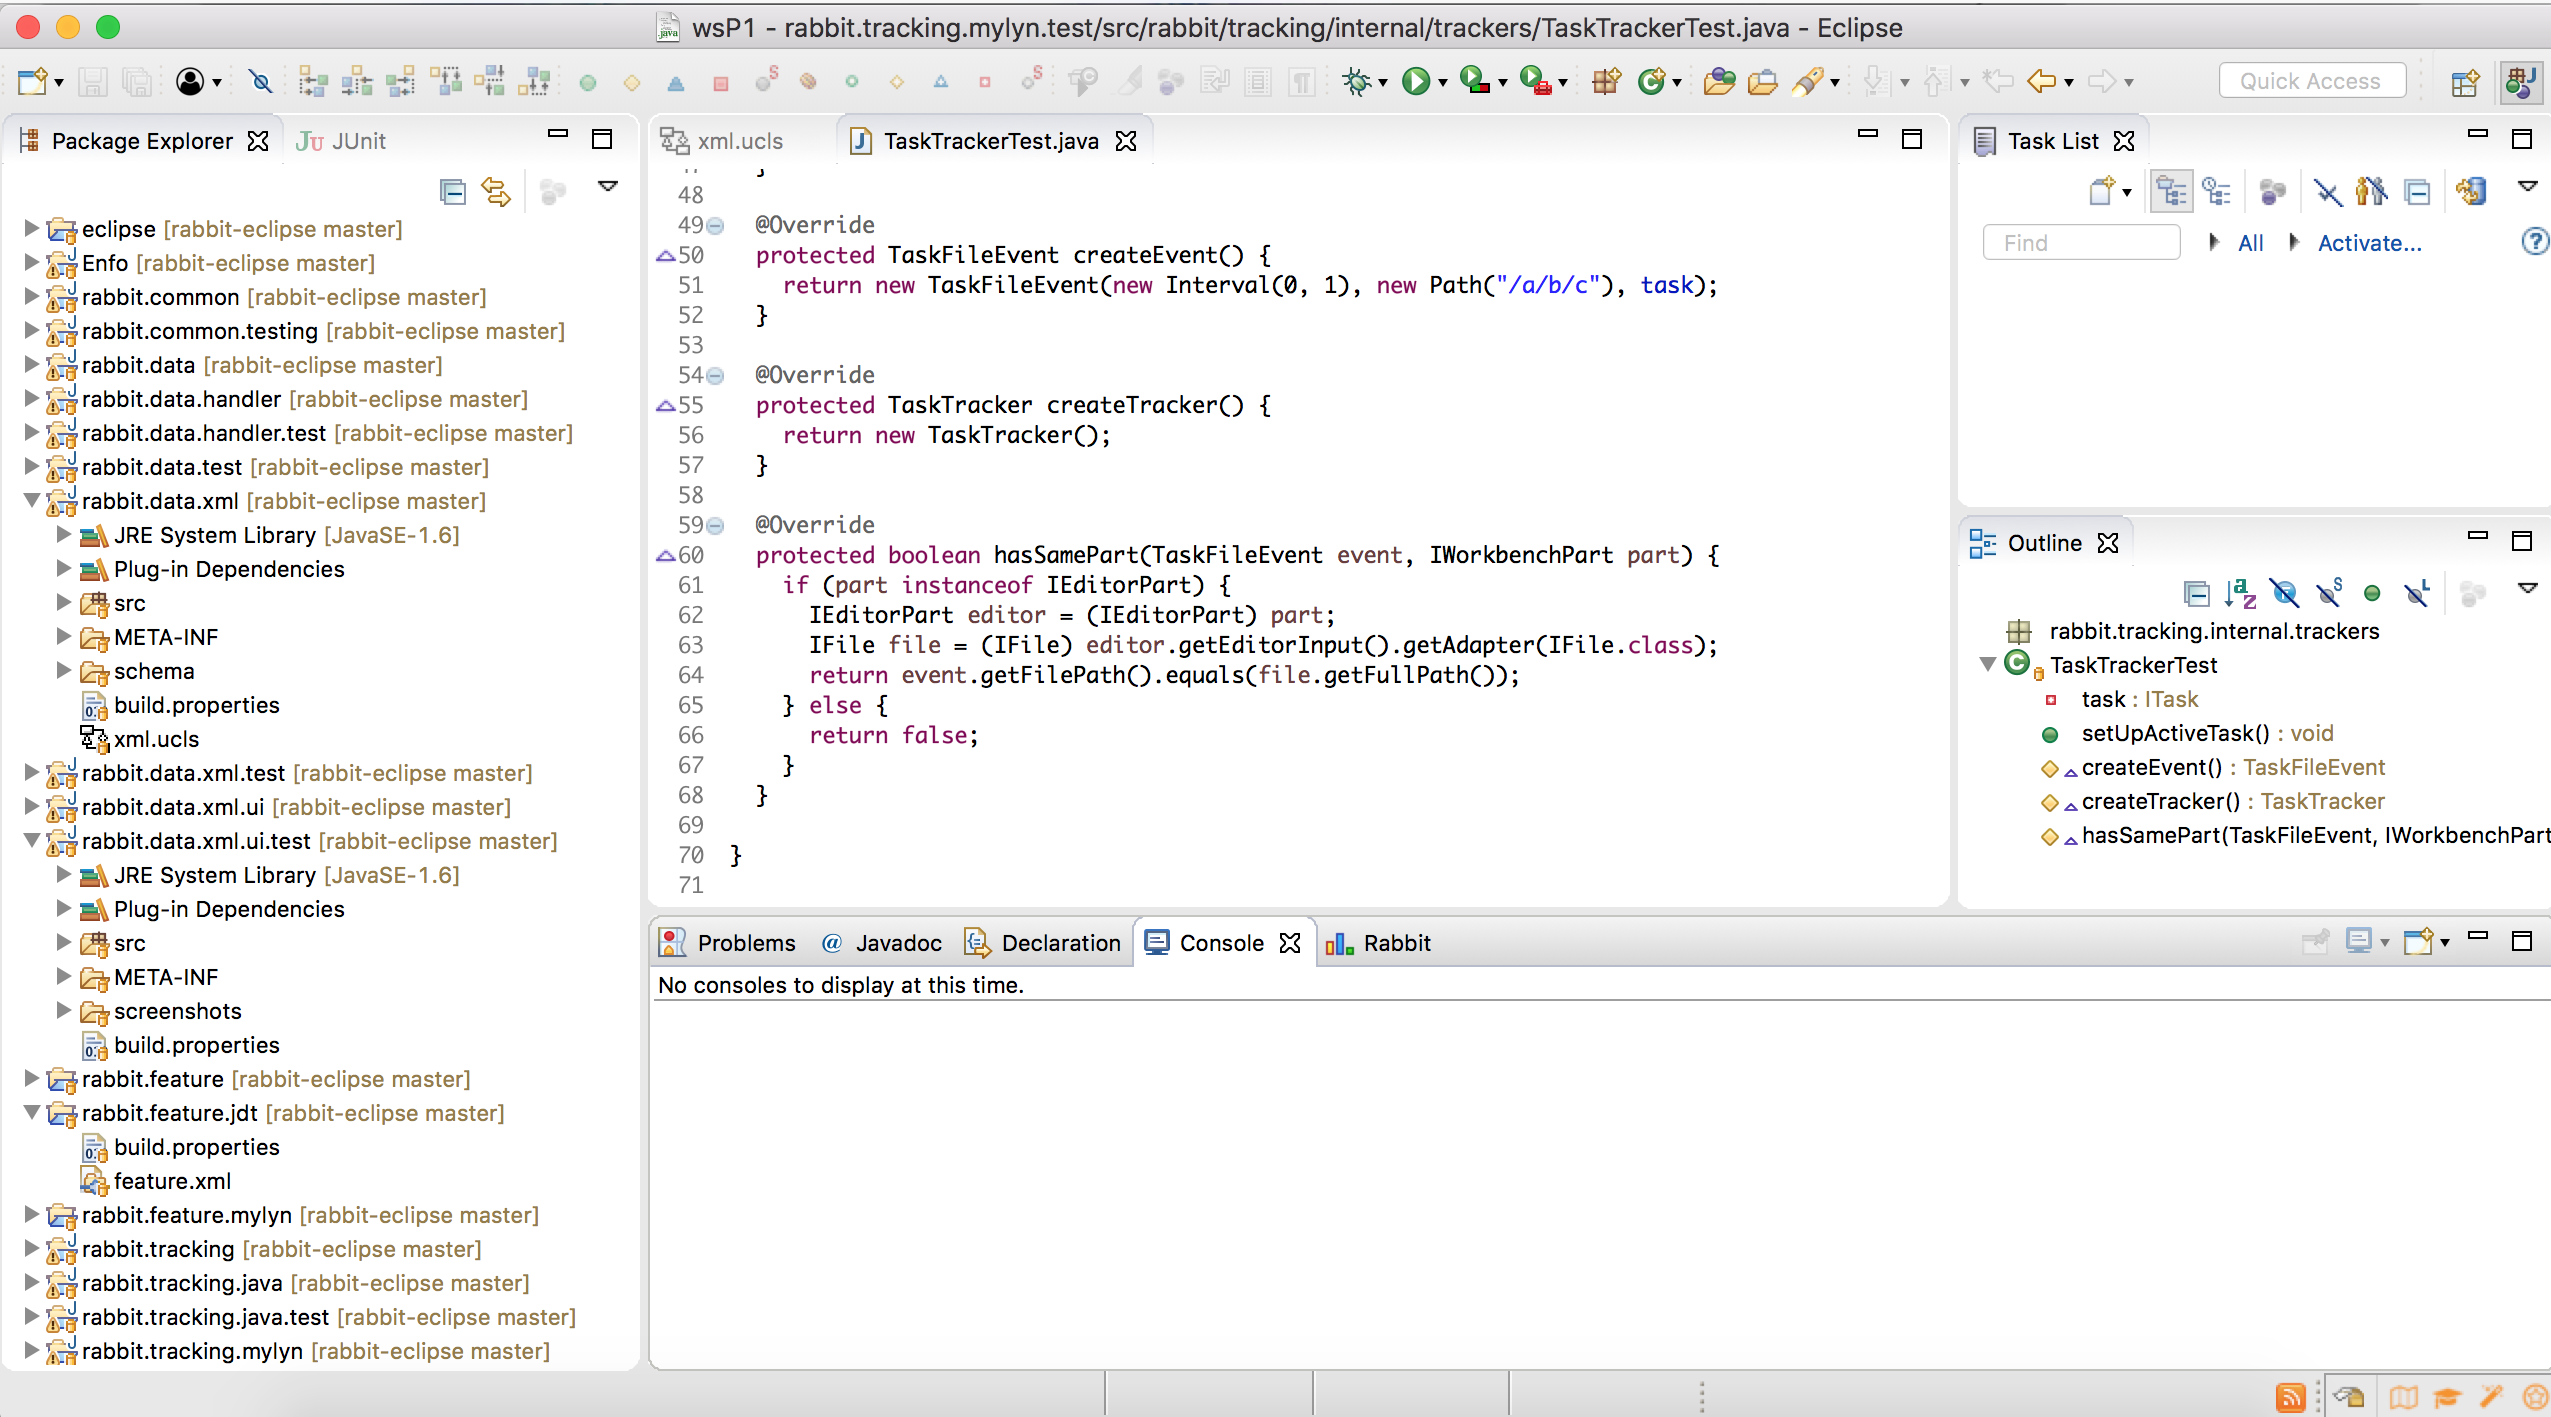
\includegraphics[width=\textwidth]{figures/eclipseWS.png}
		\end{center}
		\caption{The Java Development perspective in Eclipse.}
		\label{fig:eclipse_workspace}
	\end{figure}
A \textit{view} is a window that enables the developer to examine something, eclipse offers various of views f.x. Java packages and their files. An \textit{editor} is a smart editor which recognizes the programming language markups the syntax and allows you to modify and save files. Editors share characteristics with views, but unlike views, editors don't have tool-bars. Eclipse is filled up with \textit{menus}, the main menu is at the top of the screen while views and explorers usually provide their own context menus.

Eclipse \gls{ide} is highly adjustable and enables the developer to construct and save his own perspectives according to his preferences. Having these advantages in mind one can optimise working capabilities.

\subsection{A closer look to Eclipse}
A closer look into Eclipse and how it works is provided. Each workbench is consisted by several windows as mentioned. These windows have their own selection service instance to be handled. The selection service instances are responsible to track selection activity and to propagate selection changes to all registered listeners. Selection events can be triggered either through user interaction or programmatically, and they occur when the selection in the current active part is changed or when a different part is activated. 

The view where elements or text is selected does not need to know who is interested in the selection. This gives the capability of creating new views that depend on the selection of an existing view without changing the context of the existing view.

The next sections explain who provides what kind of selections to whom.




\section{Plug-ins}
\label{sec:TheEclipseIDE:plug-ins}

\subsection{Plug-in Structure}
Eclipse is a multifunction framework and it provides several software components (plug-ins). Eclipse Marketplace client gives the advantage of searching, and discovering popular extensions for developers to enhance their working environment. Eclipse is based on the OSGi technology, and the software components are usually packaged and distributed as OSGi bundles. OSGi bundles are very similar to standard JAR packages. An OSGi bundle must contain a manifest file with the mandatory metadata.\addref{Richard hall et al osgi in action creating modular applications in java 1st greenwich ct usa manning publication co 2011 isbn 1933988916, 9781933988917}. This metadata includes a name, version, activator, dependencies, API, etc. 

The \gls{pde} enables developers to extend their Eclipse \gls{ide} by creating new additional functionalities or even improve the capabilities of already implemented plug-ins. Although the reason Eclipse provides this thumping range of tools is to support developers, usually instead a chaotic environment is generated. For this reason several researchers and developers instrumented plug-ins with the aim of gathering information for developers' activity, and also to further develop \gls{rsse}s.

\subsection{Plug-in Analysis}

For this thesis the plug-ins in concern are mostly observing the usage of Eclipse artifacts and 
recording activity as well as interactions of a developer. 
Several of these type of plug-ins can be found in git-hub and the Eclipse Market, emphasize was given
to the following plug-ins:

\textbf{Fluorite} is a plug-in developed in the School of Computer Science 
at Carnegie Mellon university. Its purpose is low level event logging 
for Eclipse when using the code editor. In other words, events such as: \cite{Yoon2011}
\addref{add link http://www.cs.cmu.edu/~fluorite/} 
character type, text cursor movement, 
selected text modification, as well as, all
the other available Eclipse commands that can be called for an editor.
Fluorite could potentially be used to extract developers' coding 
activity and use to detect and measure the time for various usage 
patterns or events of interest. However, this plug-in seemed promising 
and a good candidate for process mining, it was not possible to gain 
access to its source code.
 
\textbf{Usage Data collector} is a framework for collecting information about how developers 
are using the eclipse platform. Information for views usage, editor usage, 
changes of perspectives, actions invoked are recorder by monitors which
are being used including also a timestamp. Moreover this plug-in also collects 
basic information about the runtime environment (OS, system architecture, window system, 
locale, etc). This information are uploaded periodically to servers hosted by The Eclipse 
Foundation with the purpose to be processed in a later stage \addref{https://www.eclipse.org/org/usagedata/}.
Since this plug-in records relevant information it could offer a useful structure for mining the developers workflow, 
however, due to the fact that the development stopped a long time ago, access to source code was not achieved.
The project was shut down mainly due to resource constraints. Despite the efforts of researchers, not valuable 
knowledge was obtained from the data. 
%\todo{however access to some data collected can be found and maybe is possible to do some process mining on those data}

\textbf{Metrics} is a plug-in that calculates various metrics for your code during build cycles and warns you of range violations for each metric.
\addref{https://marketplace.eclipse.org/content/eclipse-metrics}. 
Metrics examples are the number of classes, children, interfaces, depth of inheritance, overridden methods,etc.
This information can be extracted as an xml and therefore some data mining could be performed.

\textbf{Mylyn} is a subsystem in Eclipse used for task management. The original name of this project is Mylar, and was used in studies such as \addref{how are java softwaere developers usingthe eclipse IDE}
because it captures events, such as preference changes, 
perspective changes, window events, selections, periods of inactivity, commands invoked through menus or key bindings and URLs viewed through the embedded Eclipse browser.
This tool allows the developers to work in a task-focused interface, such tasks are f.x. fixing bugs, problem reports, new features.
Mylyn allows developers' tasks to be organized and monitors its activity. It provides awareness for the progress of tasks, and increases the productivity by reducing unnecessary navigation, searching and scrolling.
Further Mylyn allows the creation of graph elements and relationships of program artifacts.\\
\textbf{TimeKeeper} this plug-in was an extension to Mylyn in order to track time, and report how long a developer worked on a certain task.

\textbf{Rabbit} is a statistics tracking plug in for Eclipse. Rabbit collects data on which operation have been performed over a set period of time.
Rabbit view provides developers with information regarding their command usage (copy,paste, build) 
used as well as their tools usage (resources, perspectives, launches). The development of Rabbit was also terminated, however documentation and source code were available on github.
Rabbit was selected to further explored, more detailed analysis is provided in \addref{chapter}%\ref{cha:TheEclipseIDE:Rabbit}.

\textbf{ITrace} interfaces with an eye tracker, determines the location of eye
gaze and map to source code element

\section{summary}
                                 	%The Patmos processor
\chapter{Modelling and Analysing}\label{sec:the operating system}
\section{background what is already there for workflow}
\section{what additional features we add to rabbit}
\section{what we could achieve with process mining}
\todo{explain what capturing events, patterns of interaction could be done to show the workflow}                                 	%The Operating System
\chapter{Analysis and Discussion }\label{cha:AnalysisAndDiscusion}
\section{what we achieved with rabbit eclipse, how was it improved and why}
\section{discussion of attempts with process mined results}
\section{what workflow developers' promises, results and what can be derived}
\todo{explain what capturing events, patterns of interaction could be done to show the workflow}                                 	%Processor extension
\chapter{Conclusion}\label{cha:Conclusion}
                                 	%TiCOS extension
\appendix
%\chapter{Software Simulator of Patmos}\label{Software simulator of Patmos}

The Patmos simulator~\cite{t-crest:d2.1} is a C++ implementation made of classes and interfaces representing processor's component and is designed to be modular and extensible. A class diagram for the Patmos simulator can be seen in figure \ref{fig:patmos_simulator}.

	\begin{figure}[!ht]
		\begin{center}
		\makebox[\linewidth]{\includegraphics[scale=0.8]{figures/patmos_simulator.pdf}}
		\end{center}
		\caption{Class diagram for the Patmos software simulator}
		\label{fig:patmos_simulator}
	\end{figure}


\texttt{simulator\_t} is the main class of the simulator and controls the whole simulation. This main class must be connected to the components of the processor and so we have:

\begin{itemize}
	\item \texttt{decoder\_t}: is the component responsible for the instruction decode. The decoder translates ISA instruction and translates them to simulator instructions.
	\item \texttt{memory\_t}: abstract class for the memory, specifies a general behavior a memory should expose such as read and write operations. This abstract class is implemented by two other classes: \texttt{ideal\_memory\_t} and \texttt{fixed\_delay\_memory\_t}. The simulator uses this class to reference both processor's global and local memory.
	\item \texttt{register\_file\_t}: template class which offers methods for getting and setting each register in a group of registers. Allows to implement predicate register (\texttt{PGR}), general purpose registers (\texttt{GPR}) e special purpose registers (\texttt{SPR}).
	\item \texttt{data\_cache\_t}: another abstract class extending \texttt{memory\_t}, is the root of a hierarchy made of two other subclasses: \texttt{ideal\_data\_cache\_t} and \texttt{lru\_data\_cache\_t}. Both those classes implement a type of data cache so both wrap an other memory object to cache.
	\item \texttt{stack\_cache\_t}: another abstract class extending \texttt{memory\_t}, is the root of a hierarchy made of two other subclasses: \texttt{ideal\_stack\_cache\_t} and \texttt{block\_stack\_cache\_t}. Both those classes implement a type of stack cache and both wrap the global memory.
\end{itemize}

\texttt{instruction\_t} is another important class which wraps the concept of a processor instruction. The class offers a method for each pipeline stage (\IF, \DR, \EX, \MW) which actually executes the corresponding pipeline stage. \texttt{instruction\_data\_t} class wraps an instruction and its operands. The simulator pipeline is nothing more than a bidimensional array of \texttt{NUM\_STAGES x NUM\_SLOTS} of \texttt{instruction\allowbreak\_data\_t} objects, where \texttt{NUM\_STAGES} is the number of processor pipeline's stages and \texttt{NUM\_SLOTS} is the number of slots in each bundle.\\

The simulation is handled by a loop in the \texttt{simulator\_t} class. At each iteration a CPU cycle is executed and the following operations are performed:

\begin{enumerate}
	\item The next \texttt{NUM\_SLOTS} is decoded and the program counter is incremented (only if the \texttt{IF} pipeline stage is not stalled).
	\item For each instruction in the pipeline the method corresponding to the stage where the instruction is placed is executed.
	\item Each instruction is advanced to the next pipeline stage. In case some stage is stalled only a subset of those instructions are advanced.
	\item Memory and cache state is advanced.
\end{enumerate}

\section{Instruction Simulation}

The class \texttt{instruction\_t} is the root of a hierarchy of classes implementing each a processor instruction, this hierarchy is shown in figure \ref{instruction_hierarchy} and allows to reuse implementations common to group of instructions.

	\begin{figure}[!ht]
		\begin{center}
		\makebox[\linewidth]{\includegraphics[scale=0.6]{figures/instruction_hierarchy.pdf}}
		\end{center}
		\caption{Class diagram for simulator's instructions hierarchy}
		\label{instruction_hierarchy}
	\end{figure}

\section{Memory and Cache Simulation}

Memories, caches and memory mapped devices can be accessed through abstract classes which isolate from their actual implementation. The abstract class \texttt{memory\_t} is extended by other three abstract classes: \texttt{data\_cache\_t}, \texttt{stack\_cache\_t} and \texttt{memory\_map\_t}.

	\begin{figure}[!ht]
		\begin{center}
		\makebox[\linewidth]{\includegraphics[scale=0.7]{figures/memory_hierarchy.pdf}}
		\end{center}
		\caption{Class diagram for simulator's memory hierarchy}
		\label{memory_hierarchy}
	\end{figure}

\texttt{memory\_map\_t} extends \texttt{memory\_t} and so it offers the same interface. \texttt{memory\_map\allowbreak \_t} wraps an object of the class \texttt{memory\_t} extends its base class with a collection of \texttt{mapped\_device\_t} and offers methods to add object of this type to that collection. The class \texttt{mapped\_device\_t} represents a portion of memory which corresponds to the content of the registers of a memory mapped IO device (for example an UART). When a read/write method is called for a specific address on an object of the class \texttt{memory\_map\_t} all the \texttt{mapped\_device\_t} are inspected to look for a device having a mapped register for the address, if an object is found the read/write is forwarded otherwise the wrapped \texttt{memory\_t} is accessed. In the case of Patmos simulator the \texttt{memory\_map\_t} object is wrapped around the local memory, so memory mapped devices can be accessed through local memory read/write instructions.

                                 %Appendix A
%\chapter{ELF File Structure}

The Executable and Linking Format (\texttt{ELF}), defined in~\cite{ELF:1995}, is a standard file format used for executable files, object files and shared libraries. ELF is meant to be extensible and portable in order to make compilation and reuse of compiled code easier. ELF file format is adopted by different operating systems since it is flexible and not tied up to a particular architecture. ELF can be used to define three main types of files:
\begin{itemize}
	\item \textbf{relocatable file}: can be used to build an executable file or a shared object file, contain code and data
	\item \textbf{executable file}: contain a program and can be executed
	\item \textbf{shared object file}: is suited for compilation with relocatable files to build other shared objects or with other shared objects to build executable files
\end{itemize}

\section{File Structure}

What emerges from the ELF file types is that an object file can both be used in the linking process and in the execution itself. The same file offers different views on the data it contains in order to satisfy these requirements (as shown in figure \ref{fig:ELF file structure}).

	\begin{figure}[!ht]
        \centering
        \begin{subfigure}[b]{0.35\textwidth}
        \centering
        \includegraphics[width=\textwidth]{figures/ELF_file_structure_link.pdf}
		\caption{Linker perspective}
        \end{subfigure}%
		~\hspace{2cm}
        \begin{subfigure}[b]{0.35\textwidth}
        \centering
        \includegraphics[width=\textwidth]{figures/ELF_file_structure_ex.pdf}
		\caption{Execution perspective}
		
        \end{subfigure}%	
		\caption{ELF file structure}
		\label{fig:ELF file structure}		
	\end{figure}

\subsection{ELF Header}

The ELF header contains general information about the file that can be summarized as follows:

\begin{itemize}
	\item \texttt{e\_indent}: the first bytes are used to identify an object file
	\item \texttt{e\_type}: the type of the file, main types are: \texttt{ET\_REL} (relocatable file), \texttt{ET\_EXEC} (executable file) and \texttt{ET\_DYN} (shared object file)
	\item \texttt{e\_machine}: the architecture of the file
	\item \texttt{e\_version}: version of the object file
	\item \texttt{e\_entry}: address of the entry point of the executable, if an entry point is specified
	\item \texttt{e\_phoff}: offset in bytes of the program header table in the file
	\item \texttt{e\_shoff}: offset in bytes of the section header table in the file
	\item \texttt{e\_flags}: processor-specific flags
	\item \texttt{e\_ehsize}: size of ELF header
	\item \texttt{e\_phentsize}: size of an entry in the program's header table
	\item \texttt{e\_phnum}: number of entries in the program's header table
	\item \texttt{e\_shnum}: number of entries in the section's header table
\end{itemize}

\subsection{Program Header}

A program header table describes how to create a program from an ELF file and is needed only for executable and shared object file. A program header table is a collection of program headers each of which describes an object segment, a collection of sections.\\
A program header is a data structure made of the following fields:

\begin{itemize}
	\item \texttt{p\_type}: type of the segment, main values are:
		\begin{itemize}
			\item \texttt{PT\_NULL}: unused segment
			\item \texttt{PT\_LOAD}: loadable segment
			\item \texttt{PT\_DYNAMIC}: dynamic linking information
		\end{itemize}
	\item \texttt{p\_offset}: offset from the beginning of the file for the segment
	\item \texttt{p\_vaddr}: virtual address where the segment is located in memory
	\item \texttt{p\_addr}: physical address where the segment is located in memory
	\item \texttt{p\_filesz}: number of bytes of the segment in the file
	\item \texttt{p\_memsz}: number of bytes of the segment in memory
	\item \texttt{p\_flags}: flags for the segment
	\item \texttt{p\_align}: alignment of the segment in the file and memory, integer number (power of 2) in bytes
\end{itemize}

\subsection{Section Header}

The section header table is mandatory only for ELF files used in the linking process. Section header table contains an entry for each section in the file. Section entries contain information regarding the section like name or size.\\
All the information contained in an ELF file is divided in section, apart from ELF header, program header table and section header table.\\
An ELF sections have to meet the following requirements:
\begin{itemize} 
	\item A section must have a section header
	\item A section is hold by contiguous bytes in the file
	\item Sections do not overlap
	\item Sections may not cover all the data in the file (inactive data)
\end{itemize}

The fields contained in a section header are the following:

\begin{itemize}
	\item \texttt{sh\_name}: name of the section
	\item \texttt{sh\_type}: type of the section, describes its content
	\item \texttt{sh\_flags}: collection of 1 bit flags for the section
	\item \texttt{sh\_addr}: if the section will be loaded in memory this field contains the address of the first byte of the section in memory
	\item \texttt{sh\_offset}: the offset in byte of the first byte of the section from the beginning of the file
	\item \texttt{sh\_size}: section's size in byte
	\item \texttt{sh\_link}: section header index to link information for the section
	\item \texttt{sh\_info}: extra information about the section
	\item \texttt{sh\_addralign}: special information about alignment, may be needed by some sections
	\item \texttt{sh\_entsize}: for sections that hold a table structure this field defined the entry size
\end{itemize}

\subsubsection{Pre-defined Sections}

Some sections in an header file are pre-defined containing program and control information used by the operating system.\\
When creating an executable more object files are put together in the linking phase, the linker resolves references between object files, updates absolute references and relocates instructions. In order to do this job some extra information is needed, this information is contained in sections like \texttt{.dynamic}.\\
Pre-defined sections have reserved names beginning with a \texttt{.}, they can be:

\begin{itemize}
	\item \texttt{.bss}: holds uninitialized data and is loaded into memory and set to 0
	\item \texttt{.comment}: holds version control information
	\item \texttt{.data} and \texttt{.data1}: holds initialized data loaded into memory
	\item \texttt{.debug}: holds content for symbolic debugging purpose
	\item \texttt{.dynamic}: contains information for dynamic linking
	\item \texttt{.hash}: hash table of symbols
	\item \texttt{.line}: contains line numbering information for symbolic debugging
	\item \texttt{.note}: holds special information eventually put by vendors 
	\item \texttt{.rodata} and \texttt{.rodata1}: holds read-only values used to build the memory image of the process (non-writable data)
	\item \texttt{.shstrtab}: contains section names data
	\item \texttt{.strtab}: contains string data, usually symbols names
	\item \texttt{.symtab}: symbol table
	\item \texttt{.text}: the program's instructions
\end{itemize}
                                 %Appendix B
%-----------
% Backmatter
%-----------
\backmatter
\chaptermark{Bibliography}
\renewcommand{\sectionmark}[1]{\markright{#1}}
\sectionmark{Bibliography}
\addcontentsline{toc}{chapter}{Bibliography}        %Force addition of Bibliography to TOC
\bibliographystyle{alpha}                           %Use alpha codes for references
\bibliography{References}                           %Bibliography file called

\end{document}
% % % EOF % % %
